\section{결과 및 오류분석}

이 장은 C-BAT를 기준선과 같은 조건에서 비교하고, 오차와 경보 실패가 어떤 조건에서 생기는지 분석한다. 모든 개발 구간 결과는 f1--f4 교차검증 fold를 합산한 값이다(53일, 5,016슬롯, 피크 평가일 51일). 9월 구간은 마지막 절에서 한 번만 따로 보고한다.

\subsection{실험 설정과 성능 비교}

모든 모델은 같은 fold, 같은 결측 마스크, 같은 채점 함수로 평가했다. 비교 대상은 여섯 모델이다. B0는 지난주 같은 요일의 전력을 그대로 쓰는 단순 기준선이다. B0\_kind는 과거 28일 안에서 가동유형 $k$와 날짜유형이 같은 날 가운데 가장 최근 완전 관측일을 쓴다. M2는 생산계획을 입력으로 넣은 LightGBM\citep{ke2017lightgbm}이고, LightGBM(튜닝)은 fold 안에서 슬롯 예측과 일 피크 예측의 하이퍼파라미터를 따로 고른 판이다. 기존 BAT는 라플라스 잡음과 학습형 어텐션, 공통 잡음을 쓰는 이전 모델이고, C-BAT는 가동 상태별 가우시안 잡음과 사전 고정 어텐션을 쓰는 최종 모델이다.

지표는 목적에 맞게 나눴다. 슬롯 MAE와 WAPE는 예측 중앙값으로, RMSE와 $R^2$는 예측 평균으로 계산했다. 확률 예측의 품질은 CRPS\citep{gneiting2007scoring}로 본다. 일 피크는 예측 경로의 하루 최댓값에서 구했다. 피크 MAE는 그 중앙값으로, 피크 RMSE와 $R^2$는 평균으로 계산했다. 피크 시각 적중은 관측 피크 시각 ±2슬롯(±30분) 안에 예측 피크 시각이 들어간 비율이다. 확률 모델은 seed 0--2 결과를 평균했다.

\begin{table}[htbp]
\centering
\caption{개발 구간 f1--f4 합산 성능(53일, 5,016슬롯, 피크 51일). 단위는 kW(WAPE는 \%, 적중률은 비율). M2 행은 WAPE·$R^2$·피크 RMSE·피크 $R^2$가 저장되어 있지 않아 비워 두었다.}
\label{tab:ch4-main}
\small
\setlength{\tabcolsep}{4pt}
\begin{tabular}{lrrrrrrrrr}
\toprule
 & \multicolumn{5}{c}{슬롯} & \multicolumn{4}{c}{일 피크} \\
\cmidrule(lr){2-6}\cmidrule(lr){7-10}
모델 & MAE & RMSE & $R^2$ & WAPE & CRPS & MAE & RMSE & $R^2$ & 시각 적중 \\
\midrule
B0 & 26.84 & 52.62 & 0.280 & 29.65 & -- & 42.22 & 79.37 & $-0.058$ & 0.098 \\
B0\_kind & 8.51 & 14.98 & 0.942 & 9.40 & -- & \textbf{6.67} & \textbf{10.03} & \textbf{0.983} & 0.157 \\
M2 & 11.64 & 21.46 & -- & -- & 8.96 & 17.02 & -- & -- & 0.157 \\
LightGBM(튜닝) & 11.05 & 19.78 & 0.898 & 12.20 & 8.65 & 10.07 & 17.94 & 0.946 & 0.118 \\
기존 BAT & \textbf{7.82} & 12.61 & 0.959 & \textbf{8.64} & 6.99 & 14.50 & 16.97 & 0.952 & \textbf{0.255} \\
C-BAT & 8.50 & \textbf{12.37} & \textbf{0.960} & 9.39 & \textbf{6.96} & 8.93 & 12.07 & 0.976 & 0.203 \\
\bottomrule
\end{tabular}
\end{table}

\begin{figure}[htbp]
\centering
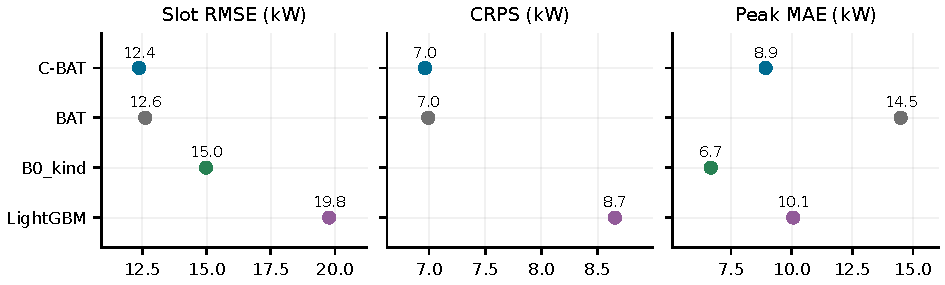
\includegraphics[width=\linewidth]{figs/model_compare.pdf}
\caption{주요 모델의 슬롯 RMSE, CRPS, 일 피크 MAE(개발 구간 f1--f4). LightGBM은 튜닝판이다.}
\label{fig:ch4-compare}
\end{figure}

C-BAT는 슬롯 곡선과 확률 예측에서 가장 좋은 축에 들고, 일 피크에서는 B0\_kind 다음이다(표~\ref{tab:ch4-main}, 그림~\ref{fig:ch4-compare}). C-BAT의 슬롯 RMSE는 12.37 kW, CRPS는 6.96 kW로 비교 모델 중 가장 낮다. 슬롯 MAE는 기존 BAT가 7.82 kW로 가장 낮고 C-BAT(8.50 kW)와 B0\_kind(8.51 kW)가 비슷하다. 생산계획을 넣은 LightGBM은 튜닝 뒤에도 슬롯 MAE 11.05 kW, CRPS 8.65 kW로 C-BAT보다 크다. B0는 슬롯 MAE 26.84 kW로 크게 뒤진다. 같은 복사 방식이라도 가동유형을 맞춘 B0\_kind는 8.51 kW이므로, 기준일을 고를 때는 가동유형 일치가 관건이다.

C-BAT의 가장 큰 개선은 일 피크에서 나온다. 기존 BAT의 피크 MAE 14.50 kW를 8.93 kW로 줄였고, 피크 $R^2$는 0.952에서 0.976으로 올랐다. 피크 MAE만 보면 B0\_kind(6.67 kW)가 가장 낮지만 다음 절에서 층별로 나눠 보면 이 차이의 성격이 달라진다. 피크 시각 적중률은 기존 BAT 0.255, C-BAT 0.203으로 모든 모델이 낮다. 피크 평가일 51일 중 13일은 최댓값 근처의 부하가 여러 시각에 걸쳐 있어 하루 최댓값이 둘 이상의 슬롯에서 같게 관측된다. 이런 날은 피크 시각을 ±30분 안에 맞히기 어렵다.

\subsection{절제와 불확실성}

짝지은 bootstrap으로 보면 C-BAT의 피크 개선은 기존 BAT와 LightGBM(튜닝)에 대해 뚜렷하다(표~\ref{tab:ch4-boot}). 차이는 C-BAT에서 비교 모델을 뺀 값이며 음수가 C-BAT에 유리하다. seed별 날짜 손실 차이를 먼저 평균한 뒤 날짜 단위로 재표집했다(B=4000). 날짜 사이 상관을 고려해 7일 블록 재표집 구간도 함께 계산했다. 기존 BAT 대비 전체 피크 MAE는 $-5.57$ kW, 고피크일 피크 MAE는 $-8.10$ kW이고 두 구간 모두 0을 포함하지 않는다. 대신 슬롯 MAE는 $+0.68$ kW 나빠졌다(구간 $[-0.01, 1.36]$). LightGBM(튜닝) 대비로는 슬롯 MAE($-2.55$ kW), CRPS($-1.69$ kW), 고피크일 피크 MAE($-13.90$ kW)가 모두 날짜 단위 구간에서 유리하다.

\begin{table}[htbp]
\centering
\caption{C-BAT와 비교 모델의 짝지은 bootstrap 차이(C-BAT $-$ 비교 모델, kW). 괄호는 날짜 단위 95\% 구간, 대괄호는 7일 블록 95\% 구간. 고피크일은 13일이다.}
\label{tab:ch4-boot}
\small
\begin{tabular}{llrll}
\toprule
비교 모델 & 지표 & 차이 & 날짜 구간 & 7일 블록 구간 \\
\midrule
기존 BAT & 슬롯 MAE & $+0.68$ & $(-0.01, 1.36)$ & $[0.34, 1.22]$ \\
 & 피크 MAE 전체 & $-5.57$ & $(-8.76, -2.07)$ & $[-12.17, -0.99]$ \\
 & 피크 MAE 고피크 & $-8.10$ & $(-11.19, -5.80)$ & $[-10.00, -5.73]$ \\
\midrule
B0\_kind & 슬롯 MAE & $-0.01$ & $(-1.27, 1.08)$ & $[-1.18, 1.21]$ \\
 & 피크 MAE 전체 & $+2.26$ & $(0.36, 4.12)$ & $[-0.29, 4.16]$ \\
 & 피크 MAE 고피크 & $-3.17$ & $(-7.04, 0.40)$ & $[-7.84, -0.11]$ \\
\midrule
LightGBM(튜닝) & 슬롯 MAE & $-2.55$ & $(-5.08, -0.33)$ & $[-7.30, 0.63]$ \\
 & 슬롯 CRPS & $-1.69$ & $(-3.48, -0.12)$ & $[-5.10, 0.68]$ \\
 & 피크 MAE 전체 & $-1.14$ & $(-3.79, 1.48)$ & $[-5.58, 2.03]$ \\
 & 피크 MAE 고피크 & $-13.90$ & $(-19.02, -9.86)$ & $[-18.59, -11.63]$ \\
\midrule
학습형 어텐션 & 슬롯 MAE & $+0.17$ & $(0.07, 0.28)$ & $[0.08, 0.23]$ \\
 & 피크 MAE 전체 & $-0.23$ & $(-0.51, -0.00)$ & $[-0.48, -0.04]$ \\
\bottomrule
\end{tabular}
\end{table}

B0\_kind는 전체 피크 MAE에서 C-BAT보다 낫다. 전체 피크 MAE는 6.67 kW 대 8.93 kW이고, 차이 $+2.26$ kW의 날짜 단위 구간 $[0.36, 4.12]$는 0을 포함하지 않는다. 반면 고피크일에서는 C-BAT가 3.17 kW 낮다. 날짜 단위 구간 $[-7.04, 0.40]$은 0을 조금 포함하지만 7일 블록 구간 $[-7.84, -0.11]$은 포함하지 않는다. B0\_kind는 가동유형이 같은 최근 날을 복사하므로 평범한 날에는 잘 맞는다. 그러나 피크가 과거보다 높게 오르는 날에는 따라가지 못한다. 요금과 설비 운용은 고피크일에 좌우되므로 이 결과를 C-BAT의 약점이자 선택 근거로 함께 적는다.

절제 비교를 보면 C-BAT의 두 설계, 곧 가동 상태별 잡음과 고정 어텐션이 피크 성능을 떠받친다(표~\ref{tab:ch4-ablation}). 공통 잡음 비교는 학습형 어텐션 모델에서만 실행했으므로 학습형 어텐션 행과 비교한다. 잡음을 상태별에서 공통으로 바꾸면 피크 MAE가 9.16 kW에서 15.29 kW로, 고피크일 피크 MAE가 4.38 kW에서 7.80 kW로 커졌다. 어텐션을 학습형으로 바꾸면 슬롯 MAE는 0.17 kW 좋아지지만 피크 MAE가 0.23 kW 나빠지고, 최대 split-$\hat R$이 1.308로 수렴 기준을 넘는다. 종류 기준 ref는 슬롯 MAE를 7.80 kW로 낮추지만 피크 MAE와 고피크일 피크 MAE가 커진다. 기존 BAT에서 생산 전달항을 빼도 슬롯 MAE 7.73 kW, 피크 MAE 14.53 kW로 기존 BAT와 거의 같았다.

\begin{table}[htbp]
\centering
\caption{절제 비교(개발 구간 f1--f4, seed 0--2 평균, kW). 공통 잡음 행은 학습형 어텐션 행과 비교한다. 기존 BAT 두 행은 split-$\hat R$ 기록이 없다.}
\label{tab:ch4-ablation}
\small
\begin{tabular}{lrrrrrr}
\toprule
모델 & 슬롯 MAE & RMSE & CRPS & 피크 MAE & 고피크 MAE & 최대 $\hat R$ \\
\midrule
C-BAT & 8.50 & 12.37 & 6.96 & \textbf{8.93} & \textbf{4.37} & 1.029 \\
학습형 어텐션 & 8.34 & \textbf{12.10} & \textbf{6.85} & 9.16 & 4.38 & 1.308 \\
공통 잡음(학습형 어텐션) & 8.26 & 12.15 & 7.43 & 15.29 & 7.80 & 2.303 \\
종류 기준 ref & 7.80 & 12.80 & 6.86 & 9.06 & 5.02 & 1.038 \\
기존 BAT & 7.82 & 12.61 & 6.99 & 14.50 & 12.47 & -- \\
기존 BAT(전이 없음) & \textbf{7.73} & 12.89 & 7.03 & 14.53 & 12.27 & -- \\
\bottomrule
\end{tabular}
\end{table}

C-BAT의 표집은 모든 fold에서 수렴 기준을 만족했다. seed 3개를 체인으로 보고 상수 모수를 뺀 22개 모수의 기본 split-$\hat R$\citep{gelman1992rhat}을 계산했다. 최댓값은 f1 내부 보정 단계의 1.029이고, 1.05를 넘은 모수는 f1--f4의 내부·외부 단계 어디에도 없었다. 이 진단은 순위 정규화 $\hat R$\citep{vehtari2021rhat}이나 꼬리 ESS가 아니므로 수렴의 충분조건은 아니다. 구간 예측은 넓은 쪽으로 치우친다. 슬롯 90\% 구간(q05--q95) 적중률은 0.990, 50\% 구간 적중률은 0.781로 명목값보다 높다. 일 피크 90\% 구간 적중률은 0.948로 명목값에 더 가깝다.

\subsection{오차와 피크가 발생하는 조건}

C-BAT의 피크 오차는 고피크일이 아니라 평범한 가동일에서 커진다(표~\ref{tab:ch4-strata}, 그림~\ref{fig:ch4-strata}). 개발 구간 51일을 비가동 14일, 가동 37일로 나누고, 관측 피크가 학습 fold의 C90을 넘은 13일을 고피크일로 따로 묶었다. C-BAT의 피크 MAE는 비가동일 2.50 kW, 가동일 11.36 kW, 고피크일 4.37 kW다. 고피크일 오차가 가동일 전체보다 작다. 기존 BAT는 비가동일 피크를 24.11 kW 높게 보았고, LightGBM(튜닝)은 고피크일을 20.37 kW 낮게 보았다. C-BAT는 두 실패를 모두 줄였지만 가동일에서 평균 $+9.74$ kW 높게 예측한다.

\begin{table}[htbp]
\centering
\caption{피크 층별 MAE와 편향(kW). 편향은 예측 평균 $-$ 관측이다. 고피크일 13일은 가동일 37일에 포함된다.}
\label{tab:ch4-strata}
\small
\begin{tabular}{lrrrrrrrr}
\toprule
 & \multicolumn{4}{c}{피크 MAE} & \multicolumn{4}{c}{피크 편향} \\
\cmidrule(lr){2-5}\cmidrule(lr){6-9}
모델 & 전체 & 비가동 & 가동 & 고피크 & 전체 & 비가동 & 가동 & 고피크 \\
\midrule
C-BAT & 8.93 & 2.50 & 11.36 & \textbf{4.37} & $+7.77$ & $+2.54$ & $+9.74$ & $-1.08$ \\
기존 BAT & 14.50 & 24.11 & 10.86 & 12.47 & $+8.10$ & $+24.59$ & $+1.87$ & $-12.24$ \\
B0\_kind & \textbf{6.67} & \textbf{0.93} & \textbf{8.84} & 7.54 & $+0.24$ & $+0.36$ & $+0.19$ & $-4.77$ \\
LightGBM(튜닝) & 10.06 & 2.51 & 12.92 & 18.27 & $+1.98$ & $+19.47$ & $-4.64$ & $-20.37$ \\
\bottomrule
\end{tabular}
\end{table}

\begin{figure}[htbp]
\centering
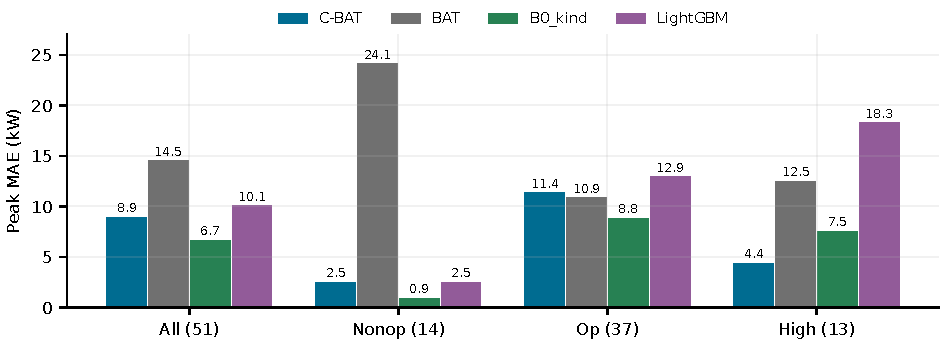
\includegraphics[width=\linewidth]{figs/peak_strata.pdf}
\caption{피크 층별 일 피크 MAE(All 51일, Nonop 비가동 14일, Op 가동 37일, High 고피크 13일).}
\label{fig:ch4-strata}
\end{figure}

슬롯 오차는 생산 시간대의 배치에서 갈린다. 가동유형별 C-BAT 슬롯 MAE는 생산 13--19시간 날 16.7 kW, 20시간 이상 날 10.0 kW, 1--12시간 날 8.2 kW, 비가동일 1.7 kW다. 13--19시간 가동일 가운데 계획상 생산이 없는 슬롯은 MAE 20.7 kW, 편향 $+13.7$ kW로 가장 나쁘다. C-BAT가 생산 시작 전이나 종료 뒤의 전력을 가동 수준으로 높게 본다. 시작 시각을 보면 07시에 시작한 2일이 21.6 kW(편향 $+17.8$ kW), 08시에 시작한 5일이 13.5 kW로, 전날부터 이어 가동하거나 01시에 시작한 날(9.4--10.4 kW)보다 크다. 하루 중에서는 18시(11.1 kW)와 19시(10.1 kW)의 오차가 가장 크고 21--23시(약 6 kW)가 가장 작다. 08--16시에는 1.4--3.8 kW 낮게 예측한다. 일 생산량 사분위별 슬롯 MAE는 10.1--11.7 kW로 차이가 작다. 요일 가운데서는 월요일이 14.1 kW(편향 $+5.2$ kW)로 가장 컸다. 그림~\ref{fig:ch4-examples}은 층별 대표일의 예측 곡선이다.

\begin{figure}[htbp]
\centering
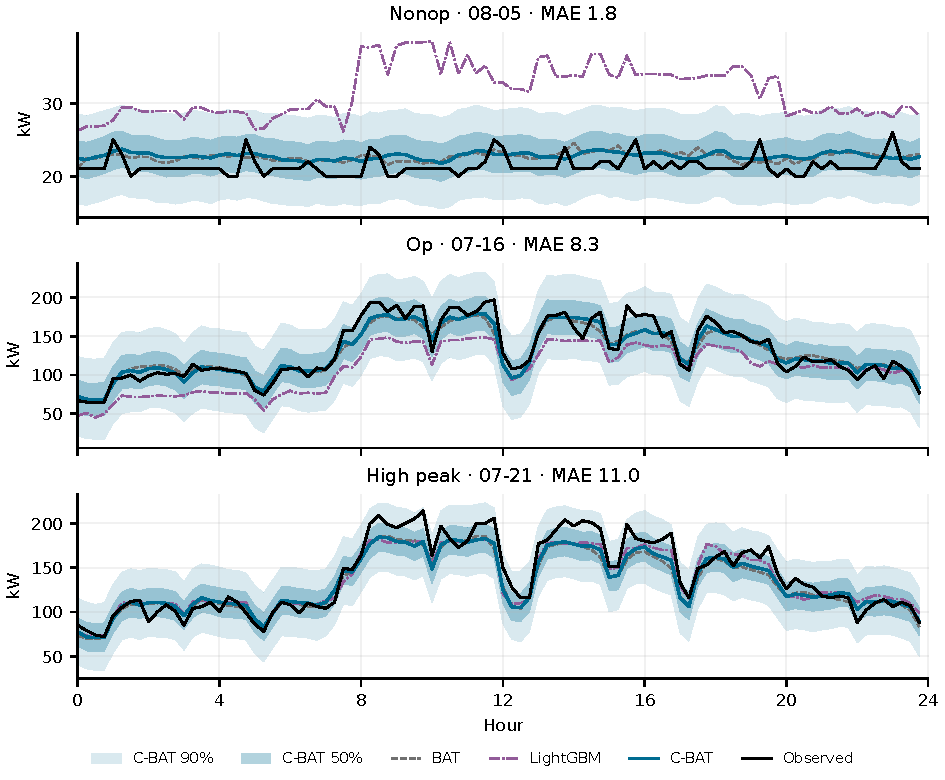
\includegraphics[width=\linewidth]{figs/forecast_examples.pdf}
\caption{층별 대표일의 C-BAT 예측(중앙값, 50\%·90\% 구간)과 관측. 대표일은 층별 일 슬롯 MAE 중앙값에 가장 가까운 날이다(seed 0).}
\label{fig:ch4-examples}
\end{figure}

실측 고피크는 긴 가동, 특정 시각, 7월에 몰렸다. 모델과 무관한 관측 사실로, 고피크일 13일은 모두 생산 13시간 이상인 날이었다(13--19시간 3일, 20시간 이상 10일). 1--12시간 가동일 5일은 평균 피크가 108 kW로 고피크가 없었다. 고피크일 13일 중 10일은 첫 최댓값이 08시(6일)나 11시(4일)에 왔고, 13일 모두 피크 시각에 생산이 계획되어 있었다. 달로 보면 7월 22일 중 11일, 8월 29일 중 2일이 고피크였다. 다만 고피크 기준인 C90이 fold마다 달라서 생긴 차이도 섞여 있다. 일 생산량은 1사분위(평균 피크 154 kW)만 낮고 2--4사분위는 199--203 kW로 비슷했다.

가동일 과대예측의 원인은 평균 곡선이 아니라 경로 최댓값에 있다. 가동일 37일에서 C-BAT 평균 곡선의 하루 최댓값은 관측 피크보다 평균 10.9 kW 낮다. 경로 최댓값의 중앙값은 여기에 약 20.1 kW를 더해, 중앙값 기준 가동일 편향이 $+9.2$ kW가 된다. 추가분은 고피크일에는 알맞다. 고피크일의 평균 곡선 최댓값은 관측보다 23.5 kW 낮고, 경로 최댓값을 쓰면 편향이 $-1.7$ kW로 줄어든다. 그러나 고피크가 아닌 가동일 24일에는 평균 곡선 최댓값의 편향이 $-4.1$ kW뿐이어서, 같은 폭을 더하면 약 $+15$ kW 과대예측이 된다. 피크 오차가 가장 큰 10일은 모두 고피크가 아닌 가동일이었고 모두 17--32 kW 과대예측이었다.

모델이 두 부류의 가동일에 서로 다른 폭을 주지 못하는 이유는 생산계획에 고피크 신호가 거의 없기 때문이다. 가동일 37일에서 C-BAT 피크 오차(중앙값 $-$ 관측, seed 평균)와 계획 특성의 상관을 계산했다. 생산 시작 시각과의 상관은 $r=-0.03$, 생산 첫 2시간의 생산량 비중과는 $r=-0.01$, 생산 시간 수와는 $r=-0.01$이었다. 계획만으로는 오차가 큰 날을 미리 가려낼 수 없다. 뒤의 확장 실험에서도 같은 결론이 되풀이된다.

\subsection{경보의 미탐지·오경보 조건}

C-BAT는 가장 드문 C90 초과에서 비교 모델보다 균형 잡힌 경보를 낸다(표~\ref{tab:ch4-alarm}). 경보는 ``오늘 피크가 기준 C를 넘는다''는 판단이다. 확률은 fold마다 내부 보정일 7일로 적합한 Platt 보정을 거쳤고, 문턱 $p^*$는 같은 fold 내부에서 F1이 가장 큰 값으로 정했다. 사건 수는 C50 31일, C75 21일, C90 13일이다. C50은 세 모델 모두 F1이 0.89 이상이다. C90에서 C-BAT의 F1은 0.584로 가장 높고 Brier 점수도 0.201로 가장 낮다. LightGBM(튜닝)은 경보를 낸 날은 모두 맞혔지만 재현율이 0.231로, 고피크 13일 중 3일만 잡았다. 매일 경보의 C90 F1(0.406)보다도 낮다.

\begin{table}[htbp]
\centering
\caption{일 피크 초과 경보 성능(개발 구간 51일, seed 평균, fold 내부 7일 Platt 보정). 매일 경보는 모든 날에 경보를 낸 기준선이다.}
\label{tab:ch4-alarm}
\small
\begin{tabular}{llrrrrr}
\toprule
기준(사건 수) & 모델 & 정밀도 & 재현율 & F1 & AUC & Brier \\
\midrule
C50 (31일) & C-BAT & 1.000 & 0.882 & 0.937 & 0.997 & 0.020 \\
 & 기존 BAT & 0.967 & 0.935 & 0.951 & 0.976 & 0.020 \\
 & LightGBM(튜닝) & 0.963 & 0.839 & 0.897 & 0.977 & 0.030 \\
 & 매일 경보 & 0.608 & 1.000 & 0.756 & -- & -- \\
\midrule
C75 (21일) & C-BAT & 0.829 & 0.921 & 0.872 & 0.844 & 0.153 \\
 & 기존 BAT & 0.769 & 0.952 & 0.851 & 0.863 & 0.211 \\
 & LightGBM(튜닝) & 0.900 & 0.429 & 0.581 & 0.798 & 0.236 \\
 & 매일 경보 & 0.412 & 1.000 & 0.583 & -- & -- \\
\midrule
C90 (13일) & C-BAT & 0.520 & 0.667 & \textbf{0.584} & 0.788 & \textbf{0.201} \\
 & 기존 BAT & 0.417 & 0.769 & 0.541 & 0.800 & 0.233 \\
 & LightGBM(튜닝) & 1.000 & 0.231 & 0.375 & 0.688 & 0.253 \\
 & 매일 경보 & 0.255 & 1.000 & 0.406 & -- & -- \\
\bottomrule
\end{tabular}
\end{table}

C90 미탐지는 7월의 종일 가동일에 몰렸다. C-BAT가 놓친 날(seed 평균 4.33일)은 모두 7월이고 모두 생산 20시간 이상인 날이었다. 그중 62\%가 일 생산량 상위 25\%였다. 7월에 생산량이 많은 종일 가동일의 피크가 학습 구간보다 높게 올라갔고, C-BAT가 그 상승 폭을 다 따라가지 못한 것으로 보인다. 오경보(seed 평균 8일)는 앞 절의 가동일 과대예측에서 나왔다. 7월과 8월이 절반씩이고, 생산 20시간 이상인 날이 62\%, 13--19시간인 날이 38\%였다. 요일로는 금요일이 38\%였고 주말 오경보는 없었다. 미탐지는 여름철 부하 상승을 늦게 따라가서, 오경보는 평범한 가동일의 피크를 높게 봐서 생긴다.

경보 수치는 보정 방식에 민감하다. fold 내부 7일 Platt 보정은 적합에 쓸 날이 적다. C-BAT의 C90 AUC는 보정 전 0.926에서 보정 뒤 0.788로 떨어졌고, Brier도 0.131에서 0.201로 나빠졌다. C75도 보정 전 Brier가 0.146으로 보정 뒤(0.153)보다 낮았다. 최종 실행에서는 8월 말 7일에 C90 초과일이 없어 보정식이 절편만 추정했고, 9월 가동일의 C90 위험이 모두 0.0013으로 고정되었다. 그래서 9월 제출 파일의 위험 확률은 보정 전 경로 확률 $P(\text{경로 최댓값} > C)$로 발행하도록 결과를 보기 전에 규칙을 정했다. 표~\ref{tab:ch4-alarm}은 이전 방식으로 계산한 개발 구간 결과이므로 모델 간 상대 비교로만 읽어야 한다.

\subsection{생산계획 입력 오차의 영향}

C-BAT는 생산량 오차에는 거의 반응하지 않고 계획 시각 오차에 더 민감하다. 학습 입력과 채점할 실제 전력은 그대로 두고 예측일에 넣는 계획만 바꿨다. 생산량 오차는 평균이 1인 로그정규 배수(σ = 0.05, 0.1, 0.2, 날짜별 10회 반복)로 넣었고, 시각 오차는 계획 전체를 1시간 앞당기거나 늦춰서 넣었다. C-BAT는 seed 0 하나로 실행했다(표집 6000회, burn-in 3000회). σ = 0.2에서도 C-BAT의 슬롯 MAE는 8.492 kW에서 8.495 kW로 0.04\% 늘었다. 계획을 1시간 이르게 넣으면 8.776 kW(+3.3\%), 늦게 넣으면 8.642 kW(+1.8\%)가 되었다. 기존 BAT(+0.44, +0.06 kW)와 LightGBM(튜닝)(+0.87, +0.69 kW)도 시각 오차에 더 민감했다. C-BAT의 피크 MAE는 모든 조건에서 8.6--8.9 kW였다. 전력이 생산량의 크기보다 가동 여부와 가동 시간대를 따른다는 앞 절의 관측과 맞는다. 현장에서는 생산량보다 가동 시작·종료 시각의 입력 정확도가 더 중요하다. 계획 취소나 설비 고장처럼 가동 여부 자체가 바뀌는 경우는 이 실험에 없다.

\subsection{9월 시험}

9월 1--14일 시험에서는 M2가 C-BAT보다 나았다(표~\ref{tab:ch4-sept}). 이 구간은 v2 개발 중에 한 번 열린 적이 있고, 동결한 C-BAT로 한 번 더 열었다. 결과를 본 뒤 모델을 고치거나 다시 돌리지 않았다. 다른 모델은 다시 적합하지 않고 저장된 예측을 같은 채점 함수로 계산했다. 관측 슬롯은 1,342개로 네 모델이 같다. 한 번 열린 구간이므로 오염되지 않은 홀드아웃이 아니며, 모델 선택 근거는 f1--f4 결과로 둔다.

\begin{table}[htbp]
\centering
\caption{9월 시험(2021-09-01--14, 14일, 1,342슬롯). Brier는 C50·C75·C90 보정 전 위험의 평균이다. 기존 BAT와 M2, B0는 v2 때 저장된 예측이다.}
\label{tab:ch4-sept}
\small
\setlength{\tabcolsep}{4pt}
\begin{tabular}{lrrrrrrrr}
\toprule
모델 & 슬롯 MAE & RMSE & $R^2$ & CRPS & 90\% 적중 & 피크 MAE & 시각 적중 & Brier \\
\midrule
B0 & 7.88 & 11.18 & 0.962 & -- & -- & 7.00 & 0.143 & 0.119 \\
M2 & \textbf{6.60} & 9.75 & 0.971 & \textbf{5.03} & 0.872 & \textbf{5.53} & 0.286 & 0.121 \\
기존 BAT & 6.82 & \textbf{9.53} & \textbf{0.972} & 5.51 & 0.948 & 7.98 & 0.286 & \textbf{0.112} \\
C-BAT & 7.18 & 9.79 & 0.971 & 5.71 & 0.984 & 8.93 & 0.286 & 0.161 \\
\bottomrule
\end{tabular}
\end{table}

C-BAT와 M2의 슬롯 MAE 차이는 표본이 작아 유의하지 않다. C-BAT $-$ M2는 $+0.58$ kW이고 날짜 단위 bootstrap 95\% 구간은 $[-0.24, 1.43]$이다. 9월에는 C90 초과일이 하루도 없어서 C-BAT의 강점인 고피크일 성능을 시험할 기회가 없었다. 대신 약점인 가동일 과대예측은 그대로 나타났다. 9월 가동일 12일의 피크 편향(중앙값 기준)은 $+10.2$ kW로, 개발 구간의 $+9.2$ kW(중앙값 기준)·$+9.7$ kW(평균 기준)와 같은 수준이다. 90\% 구간 적중률도 0.984로, 개발 구간처럼 구간이 넓다.

위험 확률은 보정 전 경로 확률로 발행했다. 규칙을 정한 뒤 한 번만 계산한 9월 Brier는 C50 0.131, C75 0.304, C90 0.047이다. 이전 7일 Platt 방식은 C75(0.111)와 C90(0.000)에서 더 낮았다. 그러나 C90의 0.000은 초과일이 없는 구간에서 위험을 상수로 꺼 버려 나온 값이고 판별력과는 관계가 없다. 보정 전 위험은 C50에서 낫고, C75·C90에서는 평범한 가동일 과대예측 때문에 위험을 높게 낸다(C90 최대 0.30).

\subsection{확장 실험과 최종 모델 선택}

C-BAT를 고친 뒤 사전 등록한 확장 실험 11가지를 f1--f4에서만 평가했고 채택된 것은 없다(표~\ref{tab:ch4-ext}). 각 실험은 결과를 보기 전에 채택 조건을 문서로 고정했다. 조건은 실험마다 조금 다르지만 공통으로 C-BAT의 전체 피크 MAE(8.93 kW)와 고피크일 피크 MAE(4.37 kW)를 지키면서 곡선이나 가동일 편향을 개선하도록 요구했다. 9월 구간은 쓰지 않았다.

\begin{table}[htbp]
\centering
\caption{사전 등록 확장 실험(개발 구간 f1--f4, seed 0--2 평균, kW). 앙상블은 C-BAT seed 0과 비교했고 fold 하나씩 뺀 가중치로 평가했다. 앙상블의 피크는 C-BAT와 같다.}
\label{tab:ch4-ext}
\small
\begin{tabular}{llrrrl}
\toprule
분류 & 변형 & 슬롯 MAE & 피크 MAE & 고피크 MAE & 불합격 사유 \\
\midrule
기준 & C-BAT & 8.50 & \textbf{8.93} & \textbf{4.37} & -- \\
\midrule
잡음 & 가동유형 4상태 & 8.76 & 9.18 & 6.50 & 가동일 편향, 고피크 \\
 & 슬롯 4상태 & 8.96 & 10.47 & 6.80 & 가동일 편향, 적중률, 고피크 \\
 & Student-$t$ 혁신 & 8.70 & 9.90 & 4.53 & 가동일 편향, 적중률 \\
 & 가동유형 + $t$ & 8.99 & 10.49 & 7.30 & 네 조건 모두 \\
\midrule
기준일 & 종류 기준(kind) & 7.80 & 9.06 & 5.02 & 전체 피크 \\
 & 계획 기준(plan) & 7.63 & 9.80 & 5.16 & 가동일 편향, 고피크 \\
 & 어텐션, 전달항 없음 & 7.92 & 11.69 & 4.85 & 전체 피크 \\
 & 어텐션 + 전달항 & 7.76 & 11.93 & 4.57 & 전체 피크 \\
\midrule
피크 계층 & v1 기준일 피크 회귀 & 7.76 & 11.85 & 21.70 & 전체 피크, 고피크 \\
 & v2 C-BAT 피크 사전 & 7.76 & 12.27 & 20.73 & 전체 피크, 고피크 \\
\midrule
앙상블 & M2 + C-BAT & 8.82 & -- & -- & 슬롯 MAE(C-BAT 8.49) \\
\bottomrule
\end{tabular}
\end{table}

확장 실험은 곡선이나 한 층만 개선했고, C-BAT의 피크 균형을 넘은 것은 없었다. 기준일을 바꾼 네 실험은 슬롯 MAE를 7.63--7.92 kW로 낮췄지만 피크 MAE가 9.06--11.93 kW로 커졌다. 어텐션 기준일 두 모형에서는 가동일 편향이 $+14.3$, $+14.7$ kW로 늘었다. 잡음 변형 4종은 구간을 넓혀 경로 최댓값을 더 끌어올렸고 가동일 편향이 $+9.38$--$+12.45$ kW로 오히려 커졌다. 전용 피크 계층은 비가동일 피크 MAE(v1 1.07 kW)와 C90 경보 F1(v1 0.686)을 개선했다. 그러나 선형 회귀가 가동일 피크를 평균 쪽으로 수축시켜 고피크일을 20 kW 넘게 낮게 보았다. M2와의 점예측 앙상블은 fold마다 고른 가중치가 0.05--0.30으로 흔들렸고, fold 하나씩 뺀 슬롯 MAE가 8.82 kW로 C-BAT(8.49 kW)보다 나빴다. 여러 방향에서 같은 결과가 나온 것은 앞에서 본 한계 때문이다. 생산계획에는 평범한 가동일과 고피크일을 가르는 정보가 거의 없어서, 곡선을 바꾸든 피크를 따로 모형화하든 한쪽을 맞추면 다른 쪽이 나빠진다.

최종 모델로 C-BAT를 고른 근거는 개발 구간의 피크 성능이다. C-BAT는 고피크일 피크 MAE 4.37 kW로 모든 비교 모델과 확장 실험 중 가장 낮고 기존 BAT와 LightGBM(튜닝) 대비 개선의 bootstrap 구간이 0을 포함하지 않는다. C90 경보의 F1과 Brier도 비교 모델 중 가장 좋다. 곡선과 구간 품질에서는 슬롯 RMSE와 CRPS가 가장 낮고 피크 90\% 구간 적중률이 0.948로 명목값에 가깝다. 여기에 경로 표본에서 초과 확률 $P(\text{경로 최댓값} > C)$를 바로 얻을 수 있어 5장의 피크 위험 운용에 쓸 수 있다. 다만 전체 피크 MAE는 B0\_kind보다 2.26 kW 크고 평범한 가동일을 약 9--10 kW 높게 예측한다. 9월 시험에서는 슬롯 MAE와 피크 MAE 모두 M2보다 나빴고, 고피크일이 없어 강점을 확인하지 못했다. 이 결과를 함께 밝히고, 5장에서는 C-BAT의 점예측보다 고피크 위험 신호를 중심으로 쓴다.
